\textbf{Question 8.} \newline
\hrule 

An engineering construction firm is currently working on power plants at three different sites. Let $A_i$ denote the event that the plant at site $i$ is completed by the contract date. Use the operations of union, intersection, and complementation to describe each of the following events in terms of $A_1, A_2,$ and $A_3$, draw a venn diagram, and shade the region corresponding to each one. \newline

First, let's write out our entire sample space. The notation I'll be using will be $C$ for completed and $N$ for not completed.
\begin{align*}
    S = \left\{ \begin{array}{cccc}
    CCC,\; CCN,\; CNN,\; CNC, \\
    NNN,\; NNC,\; NCC,\; NCN
    \end{array} \right\}
\end{align*}

Next, let's create our Venn diagram. \newline
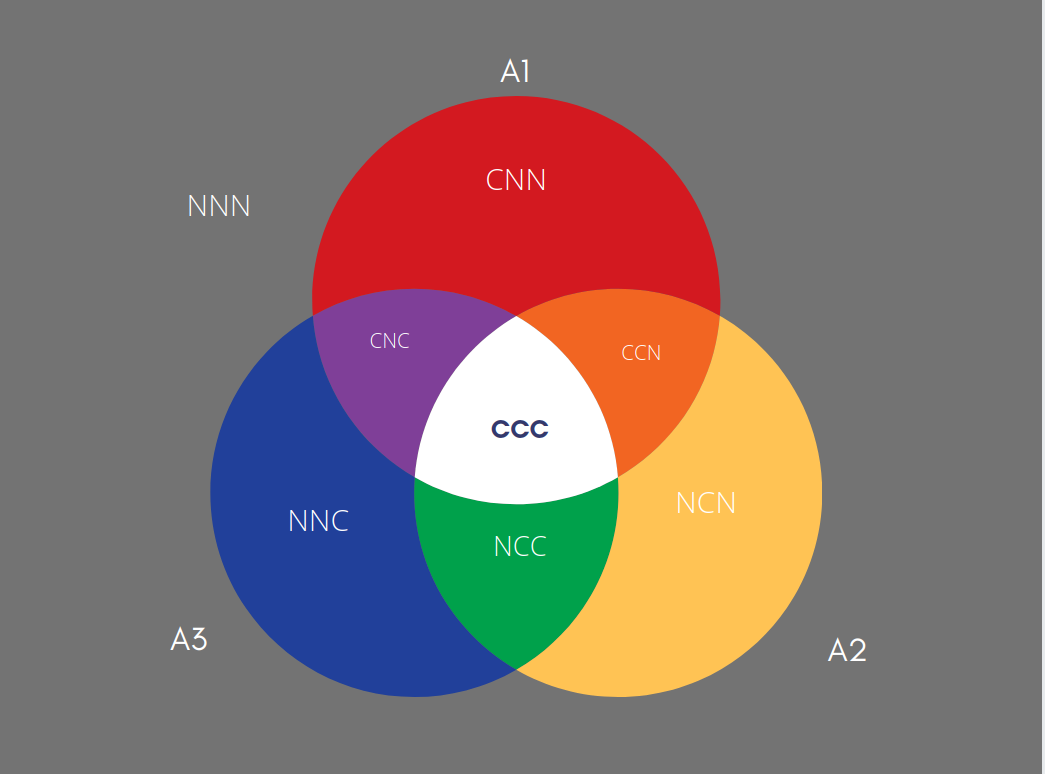
\includegraphics[scale=0.23]{images/whw3/2.1.8_venn.png}

\textbf{a. At least one plant is completed by the contract date.} \newline
This event can be described as the union between $A_1$, $A_2$, and $A_3$. In set notation this would be $(A_1 \cup A_2 \cup A_3)$. In terms of the Venn diagram, that would be everything excluding the grey outside area. 

\textbf{b. All plants are completed by the contract date.} \newline 
This event includes one single outcome, that being encompased by the white section in the center of the diagram. In terms of set notation that would be $(A_1 \cap A_2 \cap A_3)$.

\textbf{c. Only the plant at site 1 is completed by the contract date.} \newline
The red section of the Venn diagram would be the only section to fit this circumstance. I believe this can be described as $A_1$ intersecting with the intersection of $A_2'$ and $A_3'$. In other words: $(A_1 \cap (A_2' \cap A_3'))$

\textbf{d. Exactly one plant is completed by the contract date.} \newline
Using the Venn diagram, that would include the red, yellow and blue sections. The answer that came to mind is less than graceful but should work. I will neglect writing it out in words and stick entirely to set notation. \newline
$(A_1 \cap A_2' \cap A_3') \cup (A_2 \cap A_1' \cap A_3') \cup (A_3 \cap A_1' \cap A_2')$ 

\textbf{e. Either the plant at site 1 or both of the other two plants are completed by the contract date.} \newline
To explain this, our scenario here would include all 4 outcomes in $A_1$ alongside the intersection of $A_2$ and $A_3$. With the Venn diagram, that would be the red, orange, purple, white, and green sections. In set notation, that would be: \newline
$A_1 \cup (A_2 \cap A_3)$